\subsection{维纳测度}

在本号中，记 T 为 R 的区间 \([0,1]\)，记 H 为 T 上关于勒贝格测度平方可积的实函数所成的希尔伯特空间，其中内积记作 \((f|g)\)。又记 C 为 T 上在点 0 趋于 0 的连续实函数空间；赋予 C 以范数 \(\|f\| = \sup_{t \in T} |f(t)|\)。紧区间 \([0,1] = T \cup \{0\}\) 是局部紧但非紧区间 T 的 Alexandroff 紧化；因此，T 上具有紧支集的连续函数在 C 中稠密，且 C 的对偶可认作 T 上有界测度（不必为正）的空间 \(M^{1}\)（第 III 章，第 1 节，第~8号，定义 3）。

对于每个函数 \(f \in \mathcal{H}\)，由下式在 \(Pf\) 上定义函数 \(T\)：

\[
(P f) (t) = \int_ {0} ^ {t} f (x) d x = (f | \mathrm{I} _ {t}),\tag{31}
\]

其中 \(I_{t}\) 是区间 \([0, t]\) 的示性函数。柯西--施瓦茨不等式蕴含不等式

\[
| (P f) (t) | \leqslant \| f \| _ {2} \cdot t ^ {1 / 2}\tag{32}
\]

\[
\left| (P f) (t) - (P f) \left(t ^ {\prime}\right) \right| \leqslant \| f \| _ {2} \cdot \left| t - t ^ {\prime} \right| ^ {1 / 2}\tag{33}
\]

因此，\(Pf\) 属于 \(\mathcal{C}\)，且从 \(P\) 到 \(\mathcal{H}\) 的线性映射 \(\mathcal{C}\) 连续，其范数 \(\leqslant 1\)。

将希尔伯特空间 \(\mathcal{H}\) 与其对偶等同（TVS, V, §1, 第~7号，定理 3），并记 \(\Pi : \mathcal{M}^1 \to \mathcal{H}\) 为 \(P: \mathcal{H} \to \mathcal{C}\) 的转置。对于每个测度 \(\mu \in \mathcal{M}^1\) 和每个函数 \(f \in \mathcal{H}\)，有

\[
\begin{array}{r l} (\Pi \mu | f) & = \mu (P f) = \int_ {\mathrm{T}} d \mu (t) \int_ {\mathrm{T}} \mathrm{I} _ {t} (x) f (x) d x \\ & = \int_ {\mathrm{T}} f (x) d x \int_ {\mathrm{T}} \mathrm{I} _ {t} (x) d \mu (t) \end{array}
\]

由勒贝格--富比尼定理。现在，

\[
\mathrm{I} _ {t} (x) = \left\{ \begin{array}{l l} 1 & \text { if } 0 <   x \leqslant t \leqslant 1 \\ 0 & \text { otherwise }, \end{array} \right.
\]

从而最后

\[
(\Pi \mu) (x) = \mu ([ x, 1 ]) \quad \text { for } x \in \mathbf {T}.\tag{34}
\]

令 \(\mu, \nu\) 属于 \(\mathcal{M}^1\)。则

\[
\begin{array}{r l} (\Pi \mu | \Pi \nu) & = \int_ {\mathrm{T}} \Pi \mu (x) \Pi \nu (x) d x = \int_ {\mathrm{T}} d x \int_ {\mathrm{T}} \mathrm{I} _ {t} (x) d \mu (t) \int_ {\mathrm{T}} \mathrm{I} _ {t ^ {\prime}} (x) d \nu (t ^ {\prime}) \\ & = \int_ {\mathrm{T}} \int_ {\mathrm{T}} d \mu (t) d \nu (t ^ {\prime}) \int_ {\mathrm{T}} \mathrm{I} _ {t} (x) \mathrm{I} _ {t ^ {\prime}} (x) d x. \end{array}
\]

现在，\(I_{t} \cdot I_{t'}\) 是区间 \([0, t] \cap [0, t']\) 的示性函数，从而立即得到

\[
\int_ {\mathrm{T}} \mathrm{I} _ {t} (x) \mathrm{I} _ {t ^ {\prime}} (x) d x = \inf (t, t ^ {\prime}).\tag{35}
\]

于是

\[
(\Pi \mu | \Pi \nu) = \int_ {\mathrm{T}} \int_ {\mathrm{T}} \inf (t, t ^ {\prime}) d \mu (t) d \nu (t ^ {\prime}).\tag{36}
\]

根据前面的结果，由下式在 \(M^{1}\) 上定义正二次型 W：

\[
\mathrm{W} (\mu) = \int_ {\mathrm{T}} \int_ {\mathrm{T}} \inf (t, t ^ {\prime}) d \mu (t) d \mu (t ^ {\prime}) = \| \Pi \mu \| _ {2} ^ {2}.\tag{37}
\]

特别地，如果 \(t_1, \ldots, t_n\) 是 \(\mathbf{T}\) 中的元素，且 \(c_1, \ldots, c_n\) 是实数，则

\[
\mathrm{W} \left(\sum_ {j = 1} ^ {n} c _ {j} \varepsilon_ {t _ {j}}\right) = \sum_ {j, k = 1} ^ {n} c _ {j} c _ {k} \inf (t _ {j}, t _ {k})
\]

并且由于 W 为正，函数 \((t, t') \mapsto \inf(t, t')\) 是 T 上的正型核。

定理 1（Wiener）. --- 设 w 是希尔伯特空间 H 上的典范高斯投影测度在 \(P: H \to C\) 下的像。则 w 是 C 上方差为 W 的高斯测度。

按构造，\(W(\mu) = \left\|^{t} P(\mu) \right\|_{2}^{2}\)；第~5号的命题 5 表明 w 是方差为 W 的高斯投影测度。还需证明 w 是 C 上的测度。

\begin{enumerate}
\def\labelenumi{\Alph{enumi})}
\tightlist
\item
  辅助测度空间 \(^{(2)}\)（\(\Omega, m\)）的构造：
\end{enumerate}

对于每个整数 \(n \geqslant 0\)，记 \(\mathbf{D}_n\) 为形如 \(k / 2^n\)（其中 \(k = 1, 2, 3, \ldots, 2^n\)）的数的集合。置 \(\mathrm{D} = \bigcup_{n \geqslant 0} \mathrm{D}_n\)（T 中的二进

有理数集合）以及 \(\Omega = \mathbf{R}^{\mathrm{D}}\)。对于每个 \(t \in \mathrm{D}\)，记 \(\mathrm{X}(t)\) 为 \(f \mapsto f(t)\) 上的线性形式 \(\Omega\)。

对于 D 中的 \(t, t'\)，置 \(\mathbf{M}(t, t') = \inf(t, t')\)；我们已经看到 M 是 D 上的正型核。由于 D 是可数集，可以定义 \(\Omega\) 上协方差为 M 的高斯测度 m（第~6号，例 2）。

引理 3. --- 对于 D 中任意的 \(t, t'\)，

\[
\int_ {\Omega} \left| \mathrm{X} \left(\frac {t + t ^ {\prime}}{2}\right) - \frac {\mathrm{X} (t) + \mathrm{X} \left(t ^ {\prime}\right)}{2} \right| ^ {3} d m = \frac {1}{(8 \pi) ^ {1 / 2}} | t - t ^ {\prime} | ^ {3 / 2}.\tag{38}
\]

注意 \(\frac{t + t'}{2}\) 属于 D。已知（第~6号，例 2），族 \(\left(\mathrm{X}(t)\right)_{t\in \mathrm{D}}\) 是  的拓扑对偶 \(\Omega'\) 的一个基；因此存在  上的对称双线性型 ，由  刻画。按构造，\(\Omega\) 上高斯测度 m 的方差是 \(\widehat{\mathbf{M}}\) 上的二次型 \(\Omega' \times \Omega'\)\(\widehat{\mathbf{M}}\big(\mathrm{X}(t),\mathrm{X}(t')\big) = \inf(t,t')\)\(m\)\(\Omega\)\(\xi \mapsto \widehat{\mathbf{M}}(\xi ,\xi)\)。特别置\(\Omega'\)

\[
\xi = \mathrm{X} \left(\frac {t + t ^ {\prime}}{2}\right) - \frac {\mathrm{X} (t) + \mathrm{X} (t ^ {\prime})}{2};\tag{39}
\]

简单计算得

\[
\widehat {\mathbf {M}} (\xi , \xi) = \frac {| t - t ^ {\prime} |}{4}.\tag{40}
\]

由第~5号的命题 6（公式 (16)），

\[
\int_ {\Omega} | \xi | ^ {3} d m = \pi^ {- 1 / 2} 2 ^ {3 / 2} \Gamma (2) \widehat {\mathrm{M}} (\xi , \xi) ^ {3 / 2};\tag{41}
\]

由公式 (40) 和 (41) 立即得到引理。

\begin{enumerate}
\def\labelenumi{\Alph{enumi})}
\setcounter{enumi}{1}
\tightlist
\item
  从 \(u\) 到 \(\Omega\) 的映射 \(\mathcal{C}\) 的构造：
\end{enumerate}

对于每个整数 \(n \geqslant 0\)，记 \(\mathbf{E}_n\) 为 \(\mathcal{C}\) 的子空间，它由在每个区间 \(\left[\frac{k - 1}{2^n}, \frac{k}{2^n}\right]\)（\(1 \leqslant k \leqslant 2^n\)）上仿射的函数组成。\(I\)\(\mathbf{R}\) 的紧区间 I 上的仿射函数在 I 的端点处取得其界；因此，\(I\)

\[
\| f \| = \sup _ {1 \leqslant k \leqslant 2 ^ {n}} \left| f \left(\frac {k}{2 ^ {n}}\right) \right|\tag{42}
\]

对于 \(f\in \mathbf{E}_n\)

对于每个函数 \(g \in \Omega\) 和每个整数 \(n \geqslant 0\)，存在唯一一个属于 \(u_{n}(g)\) 且在 \(E_{n}\) 的每个点都与 g 一致的函数 \(D_{n}\)；记 \(T_{n}g = u_{n+1}(g) - u_{n}(g)\)。由于 \(D_{n}\) 是有限集，从 \(T_{n}\) 到 C 的映射 \(\Omega\) 连续，因而是 m-可测的。

引理 4. --- 对于每个整数 \(n \geqslant 0\)，

\[
\int_ {\Omega} \| \mathrm{T} _ {n} g \| ^ {3} d m (g) \leqslant \frac {1}{(8 \pi) ^ {1 / 2}} 2 ^ {- n / 2}.\tag{43}
\]

令 \(g \in \Omega\) 且 \(n \in \mathbf{N}\)。有 \(\mathbf{E}_n \subset \mathbf{E}_{n+1}\)；因而函数 \(T_n g\) 属于 \(\mathbf{E}_{n+1}\)，并在 \(D_n\) 的每个点为零；所以由 (42)，

\[
\left\| \mathrm{T} _ {n} g \right\| ^ {3} = \sup _ {1 \leqslant k \leqslant 2 ^ {n}} \left| \mathrm{T} _ {n} g \left(\frac {2 k - 1}{2 ^ {n + 1}}\right) \right| ^ {3} \leqslant \sum_ {k = 1} ^ {2 ^ {n}} \left| \mathrm{T} _ {n} g \left(\frac {2 k - 1}{2 ^ {n + 1}}\right) \right| ^ {3}.\tag{44}
\]

约定 \(g(0) = 0\)。通过对 g 作线性插值来构造 \(u_{n}(g)\)，可得关系\(g\)

\[
\mathrm{T} _ {n} g \left(\frac {2 k - 1}{2 ^ {n + 1}}\right) = g \left(\frac {2 k - 1}{2 ^ {n + 1}}\right) - \frac {1}{2} \left(g \left(\frac {k - 1}{2 ^ {n}}\right) + g \left(\frac {k}{2 ^ {n}}\right)\right)\tag{45}
\]

对于 \(1 \leqslant k \leqslant 2^n\)。由此通过积分得到

\[
\int_ {\Omega} \left| \mathrm{T} _ {n} g \left(\frac {2 k - 1}{2 ^ {n + 1}}\right) \right| ^ {3} d m (g) = \int_ {\Omega} \left| \mathrm{X} \left(\frac {2 k - 1}{2 ^ {n + 1}}\right) - \frac {1}{2} \left(\mathrm{X} \left(\frac {k - 1}{2 ^ {n}}\right) + \mathrm{X} \left(\frac {k}{2 ^ {n}}\right)\right) \right| ^ {3} d m;
\]

\pandocbounded{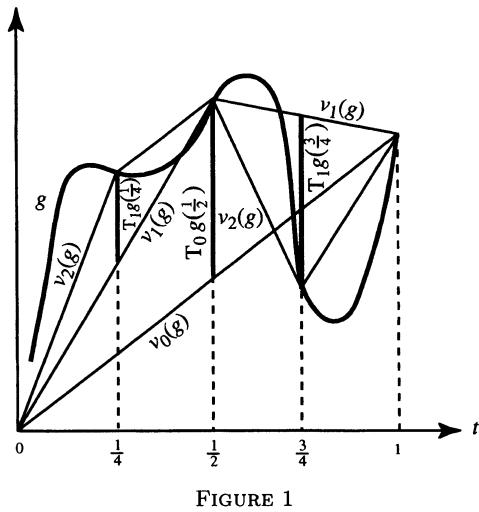
\includegraphics[keepaspectratio]{images/part002_94c2d949.jpg}}

于是可将引理 3 用于 \(t = \frac{k - 1}{2^n}\)、\(t' = \frac{k}{2^n}\)，从而

\[
\int_ {\Omega} \left| \mathrm{T} _ {n} g \left(\frac {2 k - 1}{2 ^ {n + 1}}\right) \right| ^ {3} d m (g) = \frac {1}{(8 \pi) ^ {1 / 2}} 2 ^ {- \frac {3 n}{2}}.\tag{46}
\]

由 (44)，于是有

\[
\int_ {\Omega} \| \mathrm{T} _ {n} g \| ^ {3} d m (g) \leqslant \sum_ {k = 1} ^ {2 ^ {n}} \int_ {\Omega} \left| \mathrm{T} _ {n} g \left(\frac {2 k - 1}{2 ^ {n + 1}}\right) \right| ^ {3} d m (g) = \frac {1}{(8 \pi) ^ {1 / 2}} 2 ^ {n} \cdot 2 ^ {- \frac {3 n}{2}},
\]

因而引理得证。

根据引理 4，从 \(\mathbf{T}_n\)\(\Omega\) 到巴拿赫空间 \(\mathcal{C}\) 的映射  属于 \(\mathrm{L}_{\mathcal{C}}^3 (\Omega ,m)\)，且 \(\mathrm{N}_3(\mathrm{T}_n)\leqslant \frac{1}{(8\pi)^{1 / 6}} (2^{-1 / 6})^n\)，从而 \(\sum_{n = 0}^{\infty}\mathrm{N}_3(\mathrm{T}_n) < + \infty\)。由第 IV 章第 3 节第~3号的命题 6，存在集合 \(\Omega_0\subset \Omega\)，使得 \(\Omega -\Omega_0\) 是 \(m\)-可忽略的，并且对每个 ，级数 \(\sum_{n = 0}^{\infty}\mathrm{T}_n(g)\) 在 \(\mathcal{C}\) 中绝对收敛。于是由下式定义从 \(g\in \Omega_0\)\(m\)\(u\)\(\Omega\) 到 \(\mathcal{C}\) 的 m-可测映射 ：

\[
u (g) = \left\{ \begin{array}{c l} \sum_ {n = 0} ^ {\infty} \mathrm{T} _ {n} g = \lim _ {n \to \infty} u _ {n} (g) & \text { for } g \in \Omega_ {0} \\ 0 & \text { for } g \in \Omega - \Omega_ {0}. \end{array} \right.\tag{47}
\]

由于当  时，\(u_{n}(g)\) 和 g 在 \(g\)\(\mathbf{D}_m \subset \mathbf{D}_n\) 上一致，显然对每个 \(0 \leqslant m \leqslant n\)，\(u(g)\) 在 \(\mathbf{D}\) 上的限制等于 g。\(g\)\(g \in \Omega_0\)

\begin{enumerate}
\def\labelenumi{\Alph{enumi})}
\setcounter{enumi}{2}
\tightlist
\item
  \(\mathcal{C}\) 上的高斯测度的构造：
\end{enumerate}

令 \(w'\) 为 \(\mathcal{C}\) 上的有界测度，它是 m 在 m-可测映射 \(m\)\(m\)\(u: \Omega \to \mathcal{C}\) 下的像。我们将证明 w' 是 \(w'\)\(\mathcal{C}\) 上方差为 W 的高斯测度，从而 w = w'。记 \(W\)\(w = w'\)\(\mathcal{D}\) 为 \(\mathcal{M}^1\) 的线性子空间，它由 t 遍历 D 时的测度 \(\varepsilon_t\) 生成。\(t\)\(D\)

引理 5. --- 对于每个测度 \(\mu \in \mathcal{D}\)，

\[
\int_ {\mathcal {C}} e ^ {i \langle f, \mu \rangle} d w ^ {\prime} (f) = e ^ {- W (\mu) / 2}.\tag{48}
\]

置 \(\mu=c_{1}\varepsilon_{t_{1}}+c_{2}\varepsilon_{t_{2}}+\cdots+c_{n}\varepsilon_{t_{n}}\)，其中 \(t_{1},\ldots,t_{n}\) 属于 D，\(c_{1},\ldots,c_{n}\) 属于 R。对于每个 \(g\in\Omega_{0}\)，函数 \(u(g)\) 在 D 上与 g 一致；因此

\[
\langle u (g), \mu \rangle = \sum_ {j = 1} ^ {n} c _ {j} g (t _ {j}) \quad (g \in \Omega_ {0}).\tag{49}
\]

此外，

\[
\mathrm{W} (\mu) = \sum_ {j, k = 1} ^ {n} c _ {j} c _ {k} \inf (t _ {j}, t _ {k}),\tag{50}
\]

又由于 m 是 \(\Omega\) 上协方差为 M 的高斯测度，且 \(\Omega - \Omega_{0}\) 是 m-可忽略的，有

\[
\int_ {\Omega_ {0}} e ^ {i \sum_ {j = 1} ^ {n} c _ {j} g (t _ {j})} d m (g) = \exp \Big (- \frac {1}{2} \sum_ {j, k = 1} ^ {n} c _ {j} c _ {k} \inf (t _ {j}, t _ {k}) \Big).\tag{51}
\]

现在，\(\Omega - \Omega_0\) 是 \(m\)-可忽略的，且 \(w' = u(m)\)；因此

\[
\int_ {\mathcal {C}} e ^ {i \langle f, \mu \rangle} d w ^ {\prime} (f) = \int_ {\Omega_ {0}} e ^ {i \langle u (g), \mu \rangle} d m (g).\tag{52}
\]

公式 (48) 立即由公式 (49) 至 (52) 得到。

引理 6. --- 设 \(\mu \in \mathcal{M}^1\)。存在测度序列 \(\mu_n \in \mathcal{D}\)，使得对于所有 \(\mu(f) = \lim_{n \to \infty} \mu_n(f)\) 都有 \(f \in \mathcal{C}\)，且 \(\mathrm{W}(\mu) = \lim_{n \to \infty} \mathrm{W}(\mu_n)\)。

令 \(I = [0,1]\)。将 \(\mathcal{M}^1\) 上的有界测度空间 \(T = ]0,1]\) 认作 \(\mathcal{M}(I)\) 的子空间，该子空间由在 0 处不赋予任何权重的测度组成。\(^{(3)}\) 在 \(\mathcal{M}(I)\) 上赋予弱拓扑。映射 \(t \mapsto \varepsilon_t\) 从 I 到 \(\mathcal{M}(I)\) 连续（第 III 章，第 1 节，第~9号，命题 13）；由于 D 在 I 中稠密，\(\overline{\mathcal{D}}\) 的闭包 \(\mathcal{D}\) 包含所有点测度。令 A 为满足 \(\nu \in \mathcal{D}\) 的测度 \(\| \nu \| \leqslant \| \mu \|\) 的集合；测度 \(\mu\) 属于 A 的闭包（第 III 章，第 2 节，第~4号，定理 1 的推论 1）。集合 A 在 \(\mathcal{M}(I)\) 中相对紧（第 III 章，第 1 节，第~9号，命题 15），而 \(\mathcal{M}(I)\) 的紧子集是可度量化的（TVS, III, §3, 第~4号，命题 6 的推论 2，\(^{(4)}\)，以及 GT, X, §3, 第~3号，定理 1）。因此存在测度序列 \(\mu_n \in A\)，在 \(\mu\) 中收敛于 \(\mathcal{M}(I)\)。由于 \(\mathcal{C}\) 可认作 I 上在原点为零的连续函数子空间，对于所有 \(\mu(f) = \lim_{n \to \infty} \mu_n(f)\) 有 \(f \in \mathcal{C}\)。此外，由于 \(\mathcal{C}(I) \otimes \mathcal{C}(I)\) 在赋范空间 \(\mathcal{C}(I \times I)\) 中稠密（第 III 章，第 4 节，第~1号，引理 1），关系 \(\lim_{n \to \infty} \mu_n = \mu\) 和 \(\| \mu_n \| \leqslant \| \mu \|\) 蕴含 \(\lim_{n \to \infty} (\mu_n \otimes \mu_n) = \mu \otimes \mu\)（第 III 章，第 1 节，第~10号，命题 17）；由于测度 \(\mu_n\) 和 \(\mu\) 在 0 处都不赋予权重，有

\[
\begin{array}{r} \mathrm{W} (\mu_ {n}) = \int_ {\mathrm{I}} \int_ {\mathrm{I}} \inf (t, t ^ {\prime}) d \mu_ {n} (t) d \mu_ {n} (t ^ {\prime}), \\ \mathrm{W} (\mu) = \int_ {\mathrm{I}} \int_ {\mathrm{I}} \inf (t, t ^ {\prime}) d \mu (t) d \mu (t ^ {\prime}), \end{array}
\]

从而 \(\lim_{n\to \infty}\mathrm{W}(\mu_n) = \mathrm{W}(\mu)\)。

还需证明 w' 的傅里叶变换等于 \(w'\)\(e^{-\mathbf{W}/2}\)。令 \(\mu \in \mathcal{M}^1\)，按照引理 6 选择测度 \(\mu_n \in \mathcal{D}\)。测度 w' 有界，且对所有 n 都有 \(w'\)\(|e^{i\langle f,\mu_n\rangle}| = 1\)；于是由引理 5 和勒贝格收敛定理（第 IV 章，第 4 节，第~3号，定理 2）可得\(n\)

\[
\begin{array}{r l} \int_ {\mathcal {C}} e ^ {i \langle f, \mu \rangle} d w ^ {\prime} (f) & = \lim _ {n \to \infty} \int_ {\mathcal {C}} e ^ {i \langle f, \mu_ {n} \rangle} d w ^ {\prime} (f) \\ & = \lim _ {n \to \infty} e ^ {- \mathrm{W} (\mu_ {n}) / 2} = e ^ {- \mathrm{W} (\mu) / 2}. \end{array}\tag{Q.E.D.}
\]

傅里叶变换等于 \(w\)\(\mathcal{C}\)\(e^{-\mathrm{W} / 2}\) 的 \(\mathcal{C}\) 上的测度 w 称为  上的维纳测度。

备注. --- 对于 T 中的每个半开区间 \(J = ]a, b]\)，置 \(T\)\(l(J) = b - a\)（J 的长度），并记 \(J\)\(A_J\) 为  上的线性形式 \(f \mapsto f(b) - f(a)\)。可以证明，维纳测度由如下性质刻画：\(\mathcal{C}\)

令 \(J_{1},\ldots,J_{n}\) 是 T 中两两不交的半开区间。测度 w 在从 C 到 \(f\mapsto\left(\mathrm{A}_{\mathrm{J}_{1}}(f),\ldots,\mathrm{A}_{\mathrm{J}_{n}}(f)\right)\) 的线性映射 \(R^{n}\) 下的像等于 \(\gamma_{a_{1}}\otimes\cdots\otimes\gamma_{a_{n}}\)，其中当 \(a_{i}=l(J_{i})^{1/2}\) 时 \(1\leqslant i\leqslant n\)。

